\chapter{Analysis}

\section{Introduction}

\subsection{Client Identification}
My Client is Team Cambridge Cycling Club, they run cycling event around Cambridge for any one that wishes to enter. The end user of the project is the members of Team Cambridge so that results can be uploaded soon after an event, as currently only the Racing Secretary can upload results due to the complexity of the current system. The Racing Secretary is Paul Millard currently he uses computers daily for his work, he created the club website, and he maintains the current database that hold the results of each even the club holds. This is carried out on an ASUS laptop running Windows Vista 32 bit.
\subsection{Define the current system}
I was able to interview Paul Millard about the current system, Paul also was able to provide me with a specification of the current system outing how the different systems work. Both are attached in the section appendix.

The current system uses a mix of manual data entry and automatic calculation. depending on the type of the even held determines the type of calculation that needs to be made, however some of the calculations are used across multiple types of event. The competitions that Team Cambridge members are entered for is the Transmedia, Handicap 10, Circuit, Juvenile Handicap 25 (if under age 16) and Hill Climb, once a year Team Cambridge holds an open event currently due to the complexity of the results they are uploaded as a link to a  results document. 

After the event finishes Paul enter the results in to an excel spread sheet, for handicapped competitions the personal best of each rider needs to be looked up and added to the spread sheet. If any calculations that need to be executed are done by the spread sheet and are ordered. The results are then added to the current database manual. A copy of the results are uploaded to the website and the competitions that were effected by the event are updated.

Any new riders have to entered in to the database manually and some rider change the club that they ride with, if this happens then it is dealt with manually.
\subsection{Describe the problems}
The current system has lots of manual steps that can cause the process to take a long, currently it takes on average 2 hours to process and upload one set of results

The steps that could be automated is the detection of a new rider, calling of a riders personal best, any calculations and sorting of the times and uploading data to the database
\subsection{Section appendix}

The Specification supplied by Paul Millard.

\includepdf[pages={1-9}]{TCSpecification}

The interview questions and notes taken from answers.






\section{Investigation}

\subsection{The current system}

\subsubsection{Data sources and destinations}
There are currently two sources of data used in the system, the race results and the database. For any handicap events both sources of data is needed for all other event only the results are required. The only data destination is the database.

The data from the results are on a paper form that the time keepers use during the events an example of one bellow shows that there are 8 fields, name and Address, No. , Watch Time, Emergency Tel., Club, Age, Signature. Of these fields only Name, No., Watch Time, Club and Age (if the rider is under the age of 18) are recorded in the database. As for the database the only information that is needed form it is the riders personal best time

This information is used to calculate the point that the riders are awarded in the competition(s) that are relevant to the event

All of the data sources in the current database can be found bellow

\begin{figure}[H]
    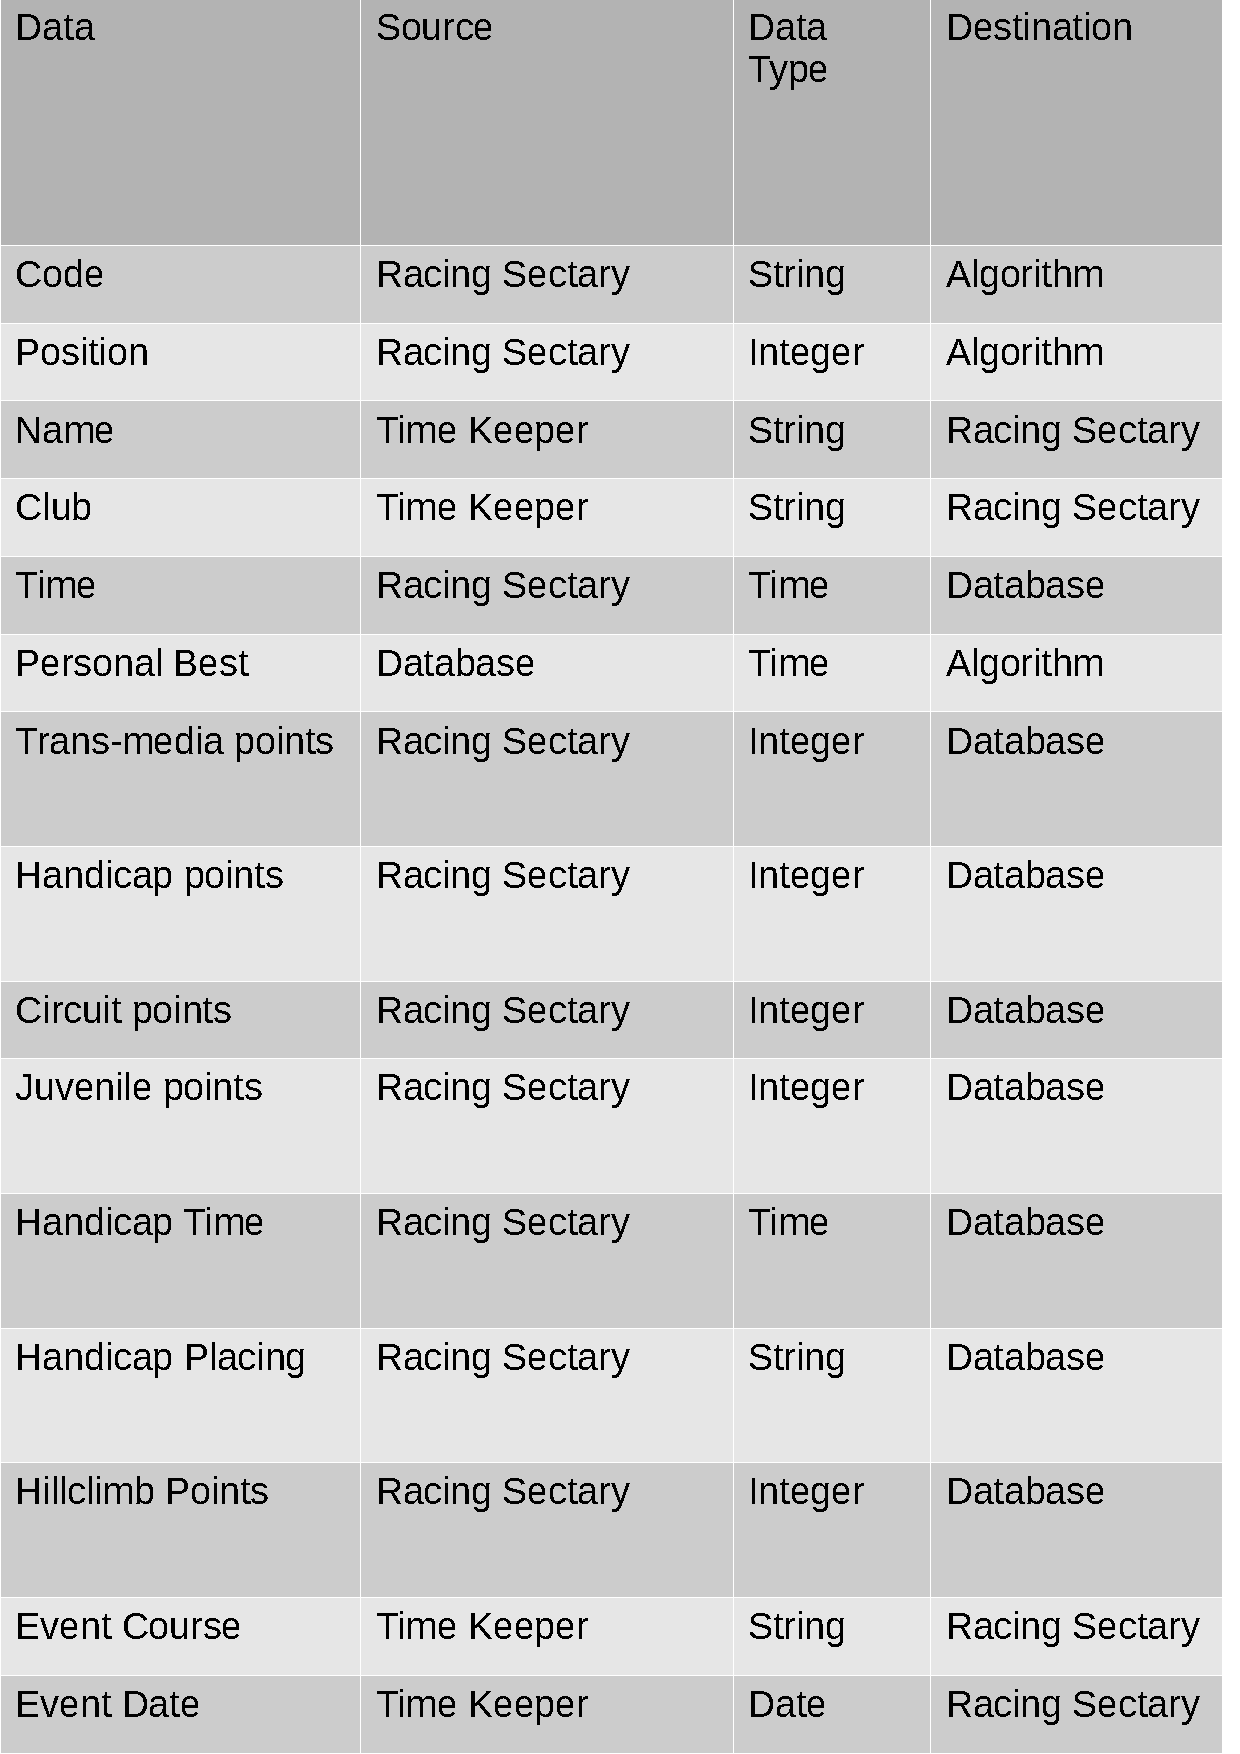
\includegraphics[width=\textwidth]{./DataSources.pdf}
    \caption{The data sources and destinations of the current system} \label{fig:Data_Sources}
\end{figure}



\subsubsection{Algorithms}
The three Algorithms that are used are shown bellow:

\begin{algorithm}[H]
\label{fig:Ride Time Algorithm}
	\caption{$Ride Time Algorithum$}
\begin{algorithmic}[1]
\SET{$Watch Time$}{$Time Value$}
\SET{$Position$}{$The Number that the rider signed on as$}
\SET{$Ride Time$}{$Watch time$}-{$Position*$}
\end{algorithmic}
\end{algorithm}

* When "Watch Time - Position" is calculated, the "Position" is treated as a time value in minuets, e.g. The rider at "Position" of 13 would have 13 minuets taken off there "Watch Time" to calculate there Ride Time"

\begin{algorithm}[H]
\label{fig:Time Sort Algorithm}
	\caption{$Time Sort Algorithm$}
\begin{algorithmic}[2]
\SET{$Times$}{$List of events Times$}
\SET{$Change$}{$True$}
\SET{$Count$}
\While{$Change$}
	\SET{$Changes$}{$False$}
	\For{$length$}{$Times$}
		\If{$Times[Count] > Times[Count + 1]$}
			\SET{$Hold$}{$Times[Count]$}
			\SET{$Times[Count]$}{$TImes[Count + 1]$}
			\SET{$Times[Count + 1]$}{$Hold$}
			\SET{$Count$}{$Count + 1$}
			\SET{$Changes$}{$True$}
		\EndIf
	\EndFor
\EndWhile
\end{algorithmic}
\end{algorithm}

\begin{algorithm}[H]
\label{fig:Handicap Time Algorithm}
	\caption{$Handicap Time Algorithm$}
\begin{algorithmic}[3]
\SET{$Ride Time$}{$Ride Time(from above)$}
\SET{$Handicap$}{$**$}
\SET{$Hndicaped Times$}{$Ride Time - Hadndicap$}
\end{algorithmic}
\end{algorithm}

**The handicap if found from the rideres best time for the distance in the kast 2 years and a look up table
\subsubsection{Data flow diagram}\i
This is the data flow diargram for add the results of a handicap event.
\begin{figure}[H]
    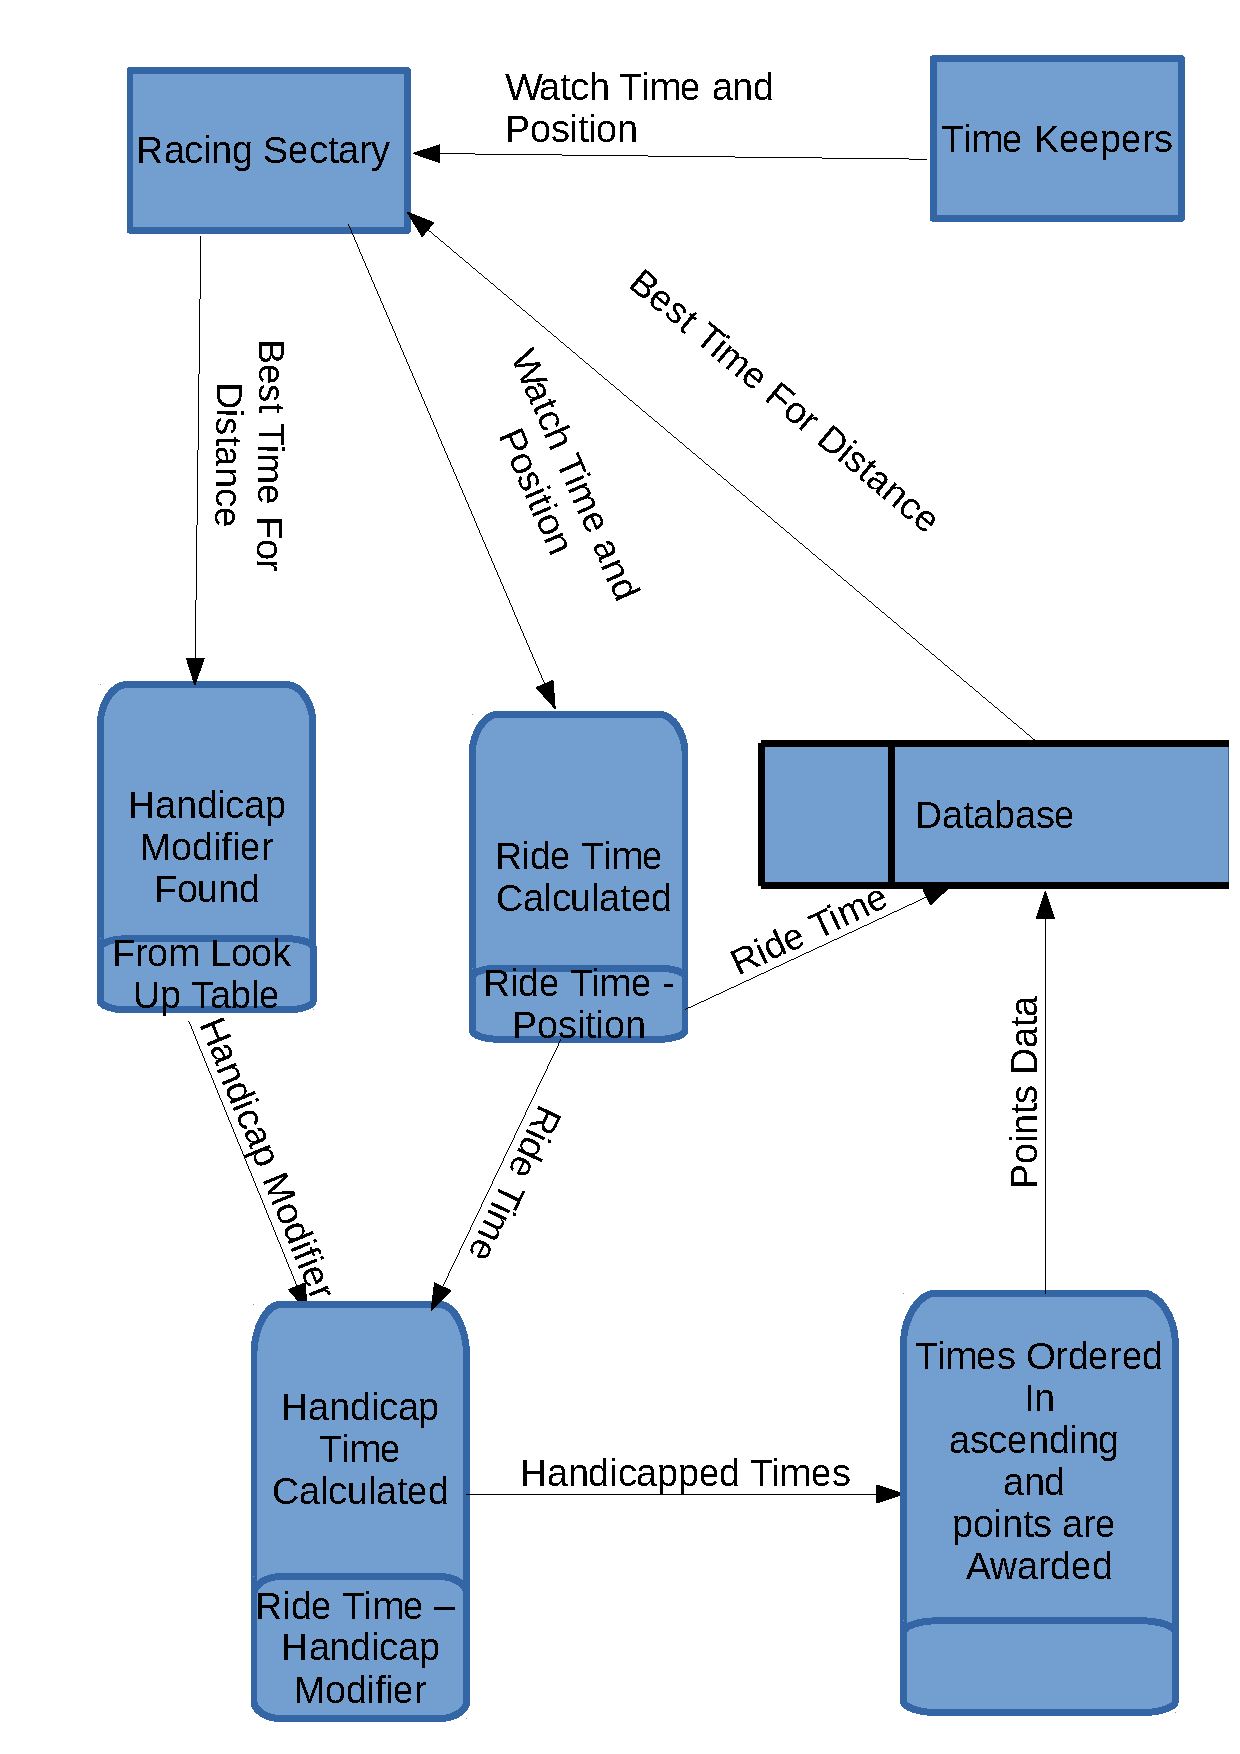
\includegraphics[width=\textwidth]{./HandicapDFD.pdf}
    \caption{Handicap events data flow diagram} \label{fig:Handicap_even_DFD}
\end{figure}

This is the data flow diargram for adding a non-handicap even.
\begin{figure}[H]
    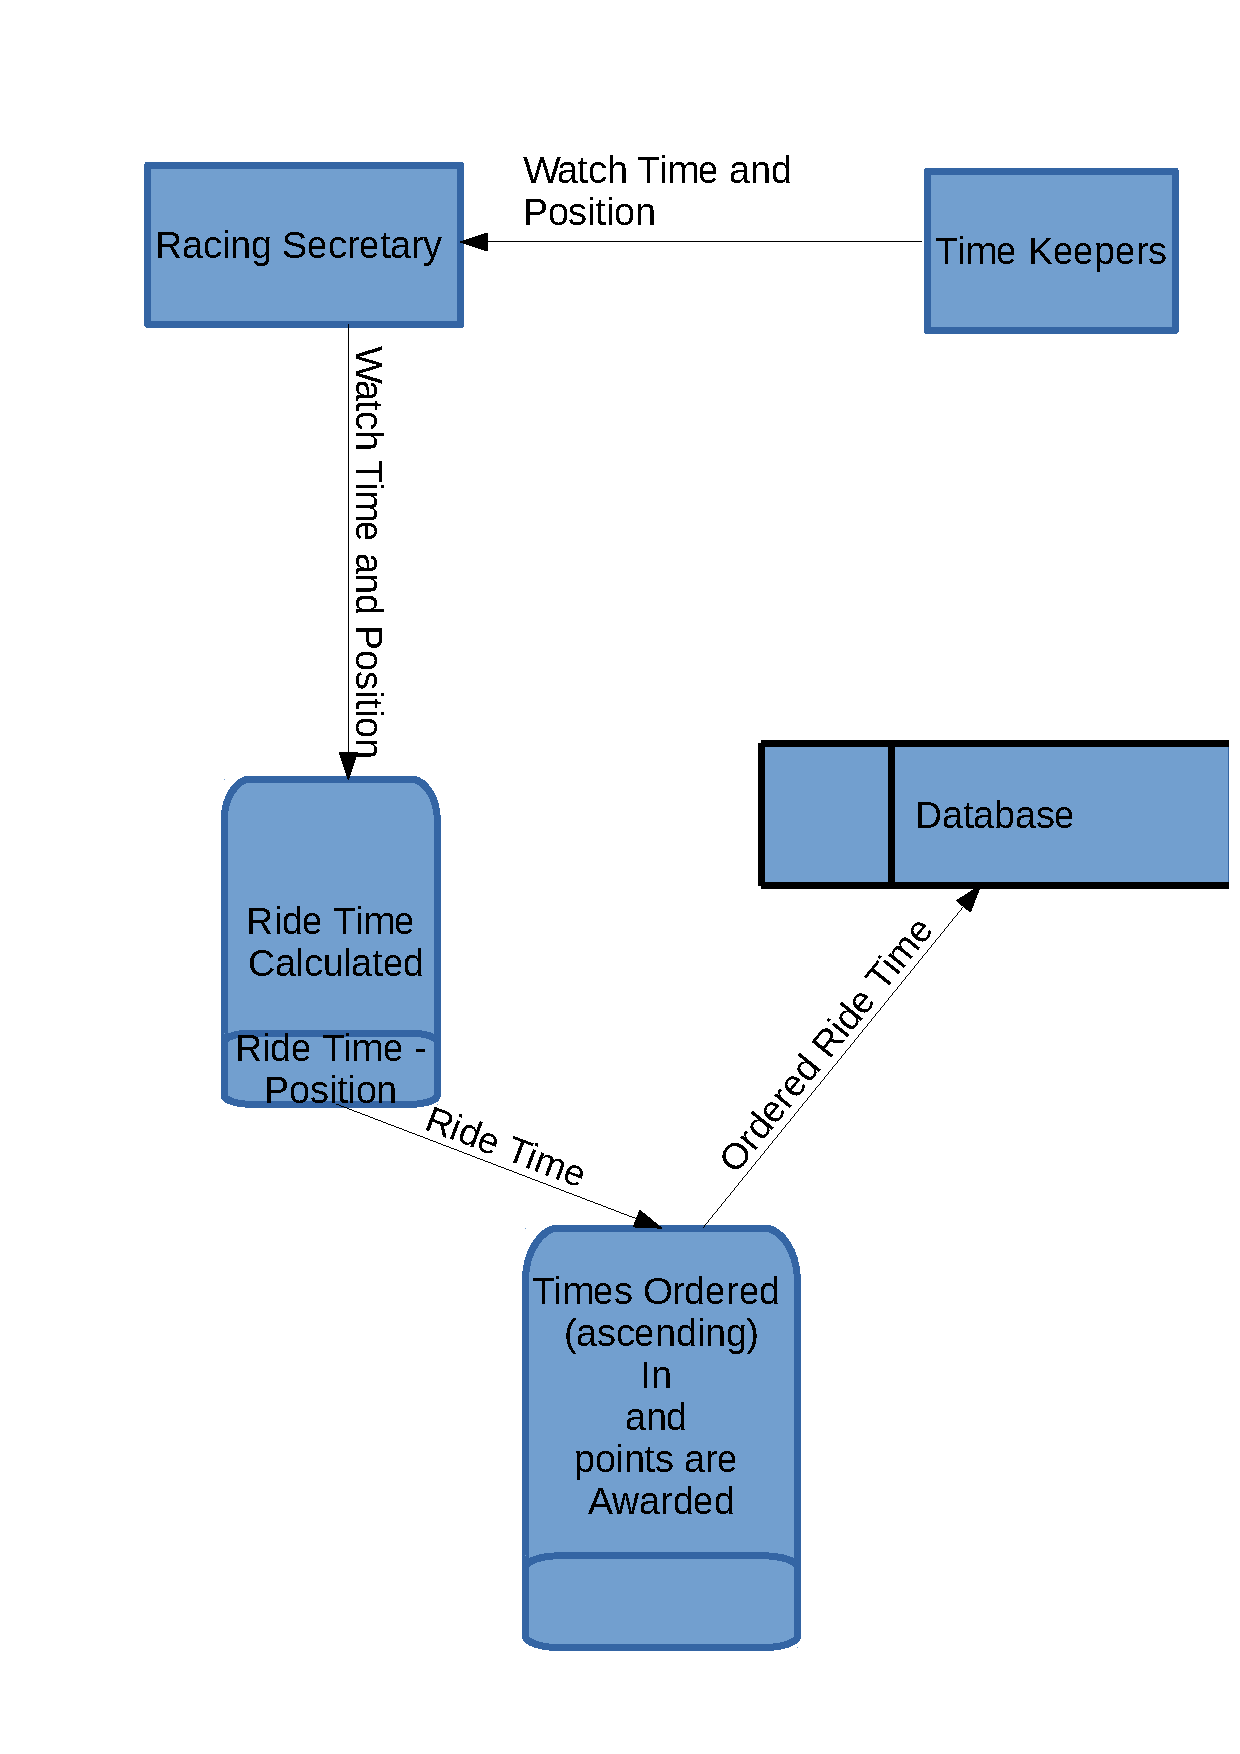
\includegraphics[width=\textwidth]{./Non-HandicapDFD.pdf}
    \caption{Non-Handicap events data flow diagram} \label{fig:non-handicap_DFD}
\end{figure}

\subsubsection{Input Forms, Output Forms, Report Formats}
The current system only has one form, the sign on sheet. It's used by the Time Keepers on the day of the event, the fields on the form are "Name", "No.", "Watch Time", "Emergency Tel.", "Club", "Age", "Signature", "Course" and "Date".

\begin{figure}[H]
    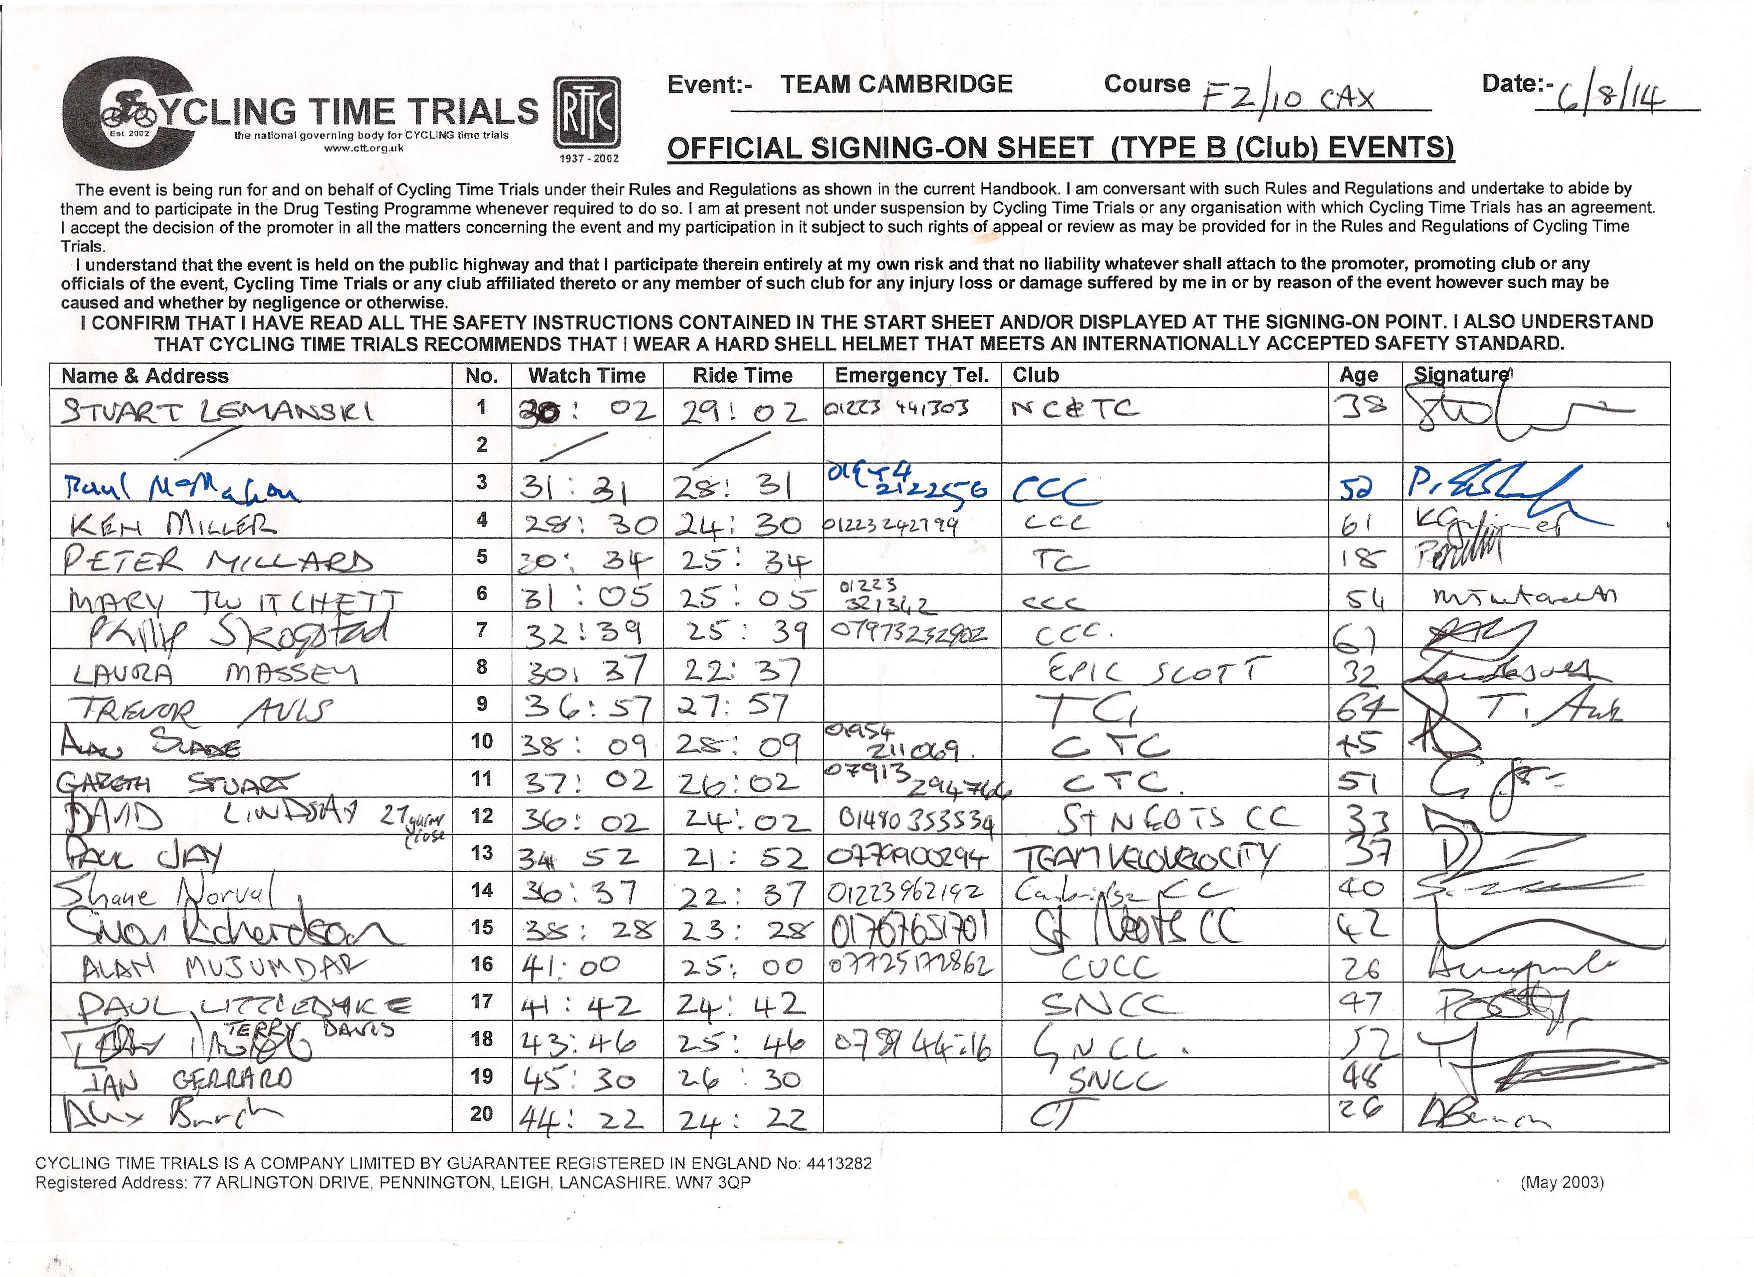
\includegraphics[width=\textwidth]{./SignOnTimeKeepersSheet.pdf}
    \caption{An example of the sign on sheet} \label{fig:Sign on Sheet}
\end{figure}
\subsection{The proposed system}

\subsubsection{Data sources and destinations}

\subsubsection{Data flow diagram}

\subsubsection{Data dictionary}

\subsubsection{Volumetrics}
Currently the raw csv files amount to 0.3 MB of data, this is approximately 7800 records. This is from partial records from 1989-1996 and then full records from 1996-present. The proposed system needs to be able to expand.
\section{Objectives}

\subsection{General Objectives}
The General objectives of the project is:
\begin{itemize}
	\item To have a web based program that's easy enough for any member to upload the even results
	\item Minimal data input
	\item Clear and simple data entry form that any user can follow
	\item The user has to be able to follow the processes
	\item The Program need to keep the minimal amount of data to keep the total amount of data in the database as low as posable
\end{itemize}

\subsection{Core Objectives}
The core objectives of the project is:
\begin{itemize}
	\item The program needs to be able to calculate times and apply the points and positions for Team Cambridge specific competitions
	\item The program needs to allow the user to edit the final data set, so any errors can be manually rectified
	\item The program needs to be able to upload the data to the Team Cambridge database
\end{itemize}
\subsection{Other Objectives}
Other objective of the project is:
\begin{itemize}
	\item To retain the current results database
	\item Identify improvements to the current data base
	\item Only retain essential data required for website users 
\end{itemize}
\section{ER Diagrams and Descriptions}

\subsection{ER Diagram}

\subsection{Entity Descriptions}

\section{Object Analysis}

\subsection{Object Listing}

\subsection{Relationship diagrams}

\subsection{Class definitions}

\section{Other Abstractions and Graphs}

\section{Constraints}

\subsection{Hardware}
The Curunt system is run off an ASUS laptop with the following system spesifcation:

\begin{itemize}
\item OS: Windows Vista 32Bit
\item CPU: Intel Celleron
\item GPU:
\item RAM: 3GB
\item Storage:
\end{itemize}

This is going to be used as the minium requerments as it should be reresntative of most members that will use this program will likely have similer or better hardware.
\subsection{Software}
The Cliant does not want there members to have to buy addishional software to allow the program to work as the program will be used by mulitple members. The only exception to this is that the Race Secarty has requested that I use the current database rarther than crease a new one, however the Race Secarty will allow me to make modifications to the current database so i can inporove it by normalization.
\subsection{Time}
The cliant hsa not set a deadline for the prject so the only time restrition is thouse set by my teacher
\subsection{User Knowledge}
The user has to be able to use the program with out any knowlage of the current system, I will assume that any user is compatent with a computor as they woulnd  trusted with the permishions assosated with the database if they could not be ttursted.
\subsection{Access restrictions}
TThe current database is controlled by permishions, as 
\section{Limitations}

\subsection{Areas which will not be included in computerisation}

\subsection{Areas considered for future computerisation}

\section{Solutions}

\subsection{Alternative solutions}

\subsection{Justification of chosen solution}
